%; whizzy chapter
% -initex iniptex -latex platex -format platex -bibtex jbibtex -fmt fmt
% 以上 whizzytex を使用する場合の設定.

%     Kansai Debian Meeting resources
%     Copyright (C) 2007 Takaya Yamashita
%     Thank you for Tokyo Debian Meeting resources

%     This program is free software; you can redistribute it and/or modify
%     it under the terms of the GNU General Public License as published by
%     the Free Software Foundation; either version 2 of the License, or
%     (at your option) any later version.

%     This program is distributed in the hope that it will be useful,
%     but WITHOUT ANY WARRANTY; without even the implied warranty of
%     MERCHANTABILITY or FITNESS FOR A PARTICULAR PURPOSE.  See the
%     GNU General Public License for more details.

%     You should have received a copy of the GNU General Public License
%     along with this program; if not, write to the Free Software
%     Foundation, Inc., 51 Franklin St, Fifth Floor, Boston, MA  02110-1301 USA

%  preview (shell-command (concat "evince " (replace-regexp-in-string "tex$" "pdf"(buffer-file-name)) "&"))
% 画像ファイルを処理するためには ebb を利用して boundingbox を作成.
%(shell-command "cd image200708; ebb *.png")

%%ここからヘッダ開始.

\documentclass[mingoth,a4paper]{jsarticle}
\usepackage{kansaimonthlyreport}
\usepackage[dvips]{xy}
\usepackage{ascmac}

% 日付を定義する, 毎月変わります.
\newcommand{\debmtgyear}{2011}
\newcommand{\debmtgdate}{22}
\newcommand{\debmtgmonth}{05}
\newcommand{\debmtgnumber}{47}

\begin{document}

\begin{titlepage}

% 毎月変更する部分, 本文の末尾も修正することをわすれずに

 第\debmtgnumber{}回 関西 Debian 勉強会資料

\vspace{2cm}

\begin{center}
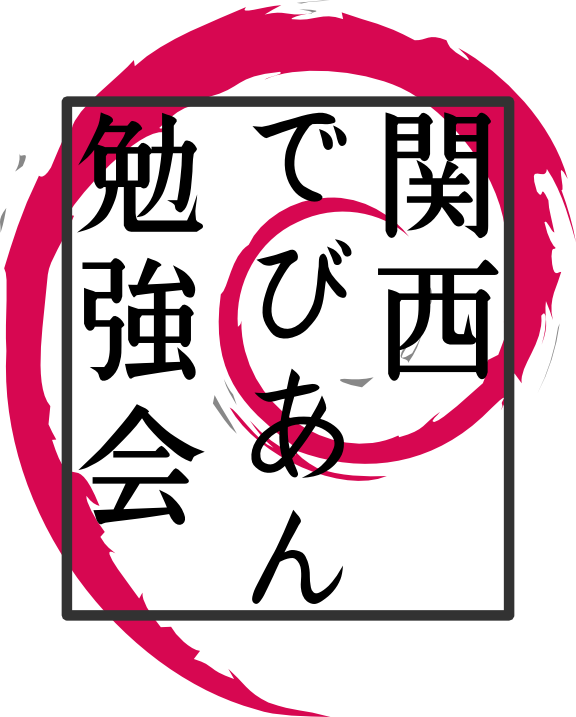
\includegraphics{image200802/kansaidebianlogo.png}
\end{center}

\begin{flushright}
\hfill{}関西 Debian 勉強会担当者 佐々木・倉敷・のがた \\
\hfill{}\debmtgyear{}年\debmtgmonth{}月\debmtgdate{}日
\end{flushright}

\thispagestyle{empty}
\end{titlepage}

\dancersection{Introduction}{Debian JP}

\subsection*{}%ロゴ用のスペース稼ぎ

関西 Debian 勉強会は Debian GNU/Linux のさまざまなトピック (新しいパッケー
ジ, Debian 特有の機能の仕組, Debian 界隈で起こった出来事, などなど) に
ついて話し合う会です.

目的として次の三つを考えています.
\begin{itemize}
      \item ML や掲示板ではなく, 直接顔を合わせる事での情報交換の促進
      \item 定期的に集まれる場所
      \item 資料の作成
\end{itemize}

それでは, 楽しい一時をお楽しみ下さい.

\clearpage

\begin{minipage}[b]{0.2\hsize}
 {\rotatebox{90}{\fontsize{80}{80}
{\gt 関西 Debian 勉強会}}}
\end{minipage}
\begin{minipage}[b]{0.8\hsize}
\hrule
\vspace{2mm}
\hrule
\setcounter{tocdepth}{1}
\tableofcontents
\vspace{2mm}
\hrule
\end{minipage}


\dancersection{最近の Debian 関係のイベント報告}{Debian JP}

\subsection{第 46 回関西 Debian 勉強会}

前回の勉強会は、4 月 16 日 (土) の OSC 2011@Kobe に参加しての開催でした。
セッションは、佐々木さんによる「遂にリリースされた(?) Squeeze について」で、
同じく佐々木さんによる GPG の基礎講座セッションもあわせて、そこそこ反響が
あったようです。

ブースには、netboot の親になれるようセッティングした squeeze マシン
を展示していたのですが、(やはりというか何というか) 一度も利用される
ことはありませんでした。

\subsection{第76回東京エリア Debian 勉強会}

丁度昨日、5 月 21 日 (土) に、東京でも Debian 勉強会が行われていました。
debian 上で apache モジュールを hack する話や、powerpc への port などが
紹介されたりしたようです。

\subsection {OSC 2011 Sendai}

同じく昨日、5 月 21 日 (土) に、仙台で OSC が開催されていました。
Debian 勉強会も参加していて、セッションはないもののブースの展示が
行われました。

\clearpage
%-------------------------------------------------------------------------------
\dancersection{事前課題}{Debian JP}

今回は以下の課題を設定しました。

\begin{quote}
  \begin{screen}
    \begin{itemize}
    \item vi 編:以下、それぞれどのようにキー操作をすれば良いか、最も少ないキー操作を考えてください。
      \begin{enumerate}
        \item 現在行から最終行(の行頭)にカーソルを移動する
        \item 現在行から最終行までを消去する
        \item 現在行から最終行までをコピー(yank)する
        \item 現在行から最終行までを "x" 1文字で置き換える
      \end{enumerate}
    \item dpkg 編
      \begin{enumerate}
        \item どれくらいの頻度で、どのような目的で dpkg コマンドや deb パッケージを直接触るか、整理してみてください
        \item パッケージ操作でやりたいのにできない、できて欲しい、といったことがあれば挙げてみてください
      \end{enumerate}
    \end{itemize}
  \end{screen}
\end{quote}

参加者の皆さんによる回答は以下の通りです。

\begin{prework}{ murase\_syuka }
  \begin{itemize}
  \item vi
    \begin{enumerate}
    \item G
    \item dG
    \item yG
    \end{enumerate}
  \item dpkg
    \begin{enumerate}
    \item インストール済みアプリの再設定
    \end{enumerate}
  \end{itemize}
\end{prework}

\begin{prework}{ 西山和広 }
  \begin{itemize}
  \item vi 編
    \begin{enumerate}
    \item G
    \item dG
    \item yG
    \item cGx \textless Esc \textgreater
    \end{enumerate}
  \item dpkg
    \begin{enumerate}
    \item dpkg -l でパッケージ一覧をみたり dpkg -L package名 でそのパッケージに含まれるファイル一覧を見たりするのはよく使います。
    \item /etc/sysctl.d などのように個別のファイルでの設定も読み込まれるようになっているものならパッケージ操作で設定の追加削除もできるのに、そうなっていないものは個別にファイル編集しかできないのが不便です。たとえば sshd\_config とか hosts.allow, hosts.deny とか。
    \end{enumerate}
  \end{itemize}
\end{prework}

\begin{prework}{ 佐藤誠 }
  \begin{itemize}
  \item Vi編 (時間がなくて探しきれていません)
    \begin{enumerate}
    \item G
    \item dG
    \item yG
    \item :., \textdollar s/* \textdollar /x/
    \end{enumerate}
  \item dpkg編
    \begin{enumerate}
    \item Debianプロジェクトによらない野良パッケージ(WebminやGoogle Chromeなど)
    \item 特にありません
    \end{enumerate}
  \end{itemize}
\end{prework}

\begin{prework}{ yabuki@netfort.gr.jp }
  \begin{itemize}
  \item vi \\viは良く知らないのでお手柔らかに。初期のモードが明示されてないので、最初に\[esc\]をおいてます。
    \begin{enumerate}
    \item [esc][shift] + g
    \item [esc]:., \textdollar d
    \item [esc]:., \textdollar y
    \item [esc]:., \textdollar s/.*/x/g
    \end{enumerate}
  \item dpkg
    \begin{enumerate}
    \item ローカルでパッケージをいじる時や、dpkg -a --configure とか、困った時。debパッケージを直接さわる時、あとは debdiffとか? mcでdebパッケージの中をみるとき?
    \item できるのかもしれないけど、/var/lib/dpkg/availableのエントリーの操作
    \end{enumerate}
  \end{itemize}
\end{prework}

\begin{prework}{ よしだともひろ }
  \begin{itemize}
  \item vi
    \begin{enumerate}
    \item G
    \item 現在行でmx(xはa〜zまでの任意の一文字)、G、\verb+:'x,.d+ ((xは上で入れた文字)
    \item 現在行でmx(xはa〜zまでの任意の一文字)、G、\verb+:'x,.y+ ((xは上で入れた文字)
    \item 現在行でmx(xはa〜zまでの任意の一文字)、G、\verb+:'x,.c+((xは上で入れた文字)[RET]、x[BS]
    \end{enumerate}
  \item dpkg
    \begin{enumerate}
    \item ごくたまにdpkg -lで入っているパッケージの確認をするぐらい
    \end{enumerate}
  \end{itemize}
\end{prework}

\begin{prework}{ かわだてつたろう }
  \begin{itemize}
  \item vi
    \begin{enumerate}
    \item G
    \item dG
    \item yG
    \item \verb+cGx<ESC>+
    \end{enumerate}
  \item dpkg
    \begin{enumerate}
    \item インストールしたパッケージの検索、パッケージ内ファイルの確認、パッケージの展開をするときに使います
    \item とくにありません
    \end{enumerate}
  \end{itemize}
\end{prework}

\begin{prework}{ kino }
  \begin{itemize}
  \item vi編
    \begin{enumerate}
    \item G
    \item d G
    \item y G
    \item \verb+:%s/^.*$/x/+
    \end{enumerate}
  \item dpkg編
    \begin{enumerate}
    \item dkpg -l | grep ....  みたいな。まだあまり使いこなせてないです。
    \item 依存関係を把握してくれつつ、checkinstall みたいにお手軽にパッケージが作れたらいいのにと思ったりします。
    \end{enumerate}
  \end{itemize}
\end{prework}

\begin{prework}{ 甲斐正三 }
  \begin{itemize}
  \item vi編
    \begin{enumerate}
    \item 「: \textdollar \textless Enter \textgreater」 (3key) or 「G」 (1key)
    \item 「:., \textdollar d \textless Enter \textgreater」 (6key) or 「dG」 (2key)
    \item 「:., \textdollar d \textless Enter \textgreater u」 (7key) or 「yG」 (2key)
    \item 第1案 「:., \textdollar d \textless Enter \textgreater ax \textless ESC \textgreater」 (9key) \\
第2案 「:., \textdollar c \textless Enter \textgreater x \textless Enter \textgreater \textless ESC \textgreater」 (9key) \\
第3案 「cGx \textless ESC \textgreater」 (4key)
    \end{enumerate}
  \item dpkg編
    \begin{enumerate}
    \item apt sources.listと違うバージョン、または存在しないパッケージ単体をダウンロードしてインストールする場合に 'dpkg' コマンドを使う。頻度は年数回程度。sources.listに加えるとややこしくなりそうなので。(実はよくわかっていない)
    \item 上記のような場合、あるリポジトリの特定のパッケージのみ依存解決、インストール、アップデートできる仕組みが欲しい。
    \end{enumerate}
  \end{itemize}
\end{prework}

\begin{prework}{ 木下 }
  \begin{itemize}
  \item vi編
    \begin{enumerate}
    \item (コマンドモード): \textdollar
    \item (コマンドモード)d:\textdollar \\
dd
    \item y: \textdollar ←最後の行はコピーできない!! \\
(コマンドモード)v \\
(最終行行末まで範囲指定) \\
y
    \item ?
    \end{enumerate}
  \item dpkg編
    \begin{enumerate}
    \item ほとんど触りません。たまにAV系コーデック等をインストールする時程度です。ほとんどapt-getです。
    \item 今は思いつきません。
    \end{enumerate}
  \end{itemize}
\end{prework}

\begin{prework}{ Kozo.Nishida }
  \begin{itemize}
  \item vi
    \begin{enumerate}
    \item G
    \item dG
    \item yG
    \item dGox
    \end{enumerate}
  \item dpkg
    \begin{enumerate}
    \item ほとんど触らない。たまにdpkg -Lするくらい
    \item 自分でdebを作ること
    \end{enumerate}
  \end{itemize}
\end{prework}

\begin{prework}{ 松澤二郎 }
  \begin{itemize}
  \item vi
    \begin{enumerate}
    \item G0
    \item dG
    \item yG
    \item cGx \textless Esc \textgreater
    \end{enumerate}
  \item dpkg
    \begin{enumerate}
    \item 気が向いたときに dpkg -l, dpkg -L を使う程度です(低頻度)。
    \item 現状に満足しています・・・(すみません)
    \end{enumerate}
  \end{itemize}
\end{prework}

\begin{prework}{ 山田 洋平 }
  \begin{itemize}
  \item vi
    \begin{enumerate}
    \item G
    \item dG
    \item yG
    \item \verb+cGx^[+
    \end{enumerate}
  \item dpkg
    \begin{enumerate}
    \item たまに dpkg -l や dpkg -L を使う程度。
    \item とくにありません。
    \end{enumerate}
  \end{itemize}
\end{prework}

\begin{prework}{ 山下康成 }
  \begin{itemize}
  \item vi 編
    \begin{enumerate}
    \item G
    \item dG
    \item yG
    \item cGx \textless ESC \textgreater
    \end{enumerate}
  \item dpkg
    \begin{enumerate}
    \item 頻度はバラバラ。dpkg -l, dpkg -P を使います
    \item X を使わないのに、無駄に X 関連のパッケージに依存していてインストールされるのがいやです。X を使わないオプションがあればいいなと思います。
    \end{enumerate}
  \end{itemize}
\end{prework}

\begin{prework}{ 八津尾 }
  \begin{itemize}
  \item vi
    \begin{enumerate}
    \item G
    \item dG
    \item yG
    \item cGx
    \end{enumerate}
  \item dpkg
    \begin{enumerate}
    \item Debian以外のディストリビューションからパッケージをひっぱってきてインストールしたい時
パッケージの設定をしたい時 \\
あのコマンドどのパッケージだっけ?という時 \\
くらいしか使いません。過去に一度だけ dpkg-buildpackage も使いました。あとはごく稀にライブラリなど取りだしたり。
    \item
    \end{enumerate}
  \end{itemize}
\end{prework}

\begin{prework}{ 小山 }
  \begin{itemize}
  \item vi編
    \begin{enumerate}
    \item 現在行で、Gコマンドを入力
    \item 現在行で、dGコマンドを入力
    \item 現在行で、yGコマンド
    \item 未回答
    \end{enumerate}
  \item dpkg
    \begin{enumerate}
    \item パッケージインストールの際、apt-getコマンドを使用するので、dpkgコマンドを使ったことはありません。
    \item 未回答
    \end{enumerate}
  \end{itemize}
\end{prework}

\begin{prework}{ 川江 }
  \begin{itemize}
  \item vi編 多分、間違ってると思いますが、
    \begin{enumerate}
    \item 1G
    \item dd
    \item yy
    \item \verb+:\%s/*/x/+ かな?
    \end{enumerate}
  \item dpkg
    \begin{enumerate}
    \item chomeをインストールするなど、debファイルを使わないとけないときに
    \item 今のところないです。
    \end{enumerate}
  \end{itemize}
\end{prework}

\begin{prework}{ tanaka jun }
  \begin{itemize}
  \item vi 編
    \begin{enumerate}
    \item G
    \item dG
    \item yG
    \item \verb+:\%s/\(.*\)/x/g+
    \end{enumerate}
  \item dpkg
    \begin{enumerate}
    \item 現在、メインで使用しているのはCentOSなので、dpkgはほとんど触りません。
    \item
    \end{enumerate}
  \end{itemize}
\end{prework}

\begin{prework}{ lurdan }
  \begin{itemize}
  \item vi
    \begin{enumerate}
    \item ]]
    \item d]]
    \item y]]
    \item \textasciicircum c]]x
    \end{enumerate}
  \item
    \begin{enumerate}
    \item ほぼ毎日、インストール済みパッケージ一覧、パッケージ内のファイル検索のために dpkg コマンドを使っています。
    \item 今のところ、特に思いつきません。
    \end{enumerate}
  \end{itemize}
\end{prework}

\begin{prework}{ oJIN }
初めて参加します。Debian 初心者です。
  \begin{itemize}
  \item
    \begin{enumerate}
    \item shift-g
    \item :., \textdollar d
    \item :., \textdollar y
    \item :., \textdollar d then x ?
    \end{enumerate}
  \item dpkg
    \begin{enumerate}
    \item printer Canon ip4600 の device driver install した時程度.
    \item CUI 環境での 日本語(editor, print)関連の導入が欲しい.
    \end{enumerate}
  \end{itemize}
\end{prework}

\begin{prework}{ ゴーインズ・ポール }

未提出

\end{prework}



\clearpage
%-------------------------------------------------------------------------------
\dancersection{ハッカーに一歩近づく Tips:vi 編}{山下康成}

\subsection{はじめに}

vi は、初心者は初心者なりに使え、使い込めば使い込むほど味の出るエディタだということは皆さんご存じの通りかと思います。
皆さんも当たり前のように vi を使ってらっしゃると思いますが、さて、ハッカーのように vi を使いこなせてますでしょうか?
ハッカーに近づくために、vi 使いこなしのちょっとした Tips を紹介します。

\subsection{こんな経験ありませんか?}

\begin{verbatim}
    k
    ↑
h ← → l
    ↓
    j
\end{verbatim}

\begin{description}
  \item[w] 一語右へカーソルを移動
  \item[G] ファイルの末尾へカーソルを移動
  \item[x] 1文字消す
  \item[dd] 1行消す
  \item[etc] ……
\end{description}

こんな教え方するから、バラバラなコマンドを覚えないとならず、なかなか「使い込めば味の出る」ところまで行けないのでしょう。今日はもうちょっと体系立てて説明してみます

\subsection{コマンドを整理してみる}

\subsubsection{繰り返し回数−コマンド 型}

回数に続いてコマンドを入力すると、指定した回数繰り返されるコマンド。
5yy として5行コピーとかは良く使われる。

例:
\begin{description}
  \item[2l] 2文字分右にカーソルを移動する
  \item[2h] 2文字分右にカーソルを移動する
  \item[2x] 2文字消す
  \item[2X] カーソルの左の2文字を消す
  \item[2r] 2文字を次に入力する文字と置き換える
  \item[2\~] 2文字を英大文字 \textless - \textgreater 小文字を切り替える

  \item[3w] 3ワード右にカーソルを移動する
  \item[3W] 空白区切りで 3 ワード右にカーソルを移動する
  \item[3b] 3ワード左にカーソルを移動する
  \item[3B] 空白区切りで 3 ワード左にカーソルを移動する

  \item[4yy] 4行コピーする
  \item[4dd] 4行削除する

  \item[5p] 5回ペーストする
  \item[5P] カーソルの前に5回ペーストする
  \item[5i \textless string \textgreater [ESC]] カーソルの左に \textless string \textgreater を5回入力する
  \item[5I \textless string \textgreater [ESC]] 行頭に \textless string \textgreater を5回入力する
  \item[5a \textless string \textgreater [ESC]] カーソルの右に \textless string \textgreater を5回入力する
  \item[5A \textless string \textgreater [ESC]] 行末に \textless string \textgreater を5回入力する
  \item[5H] 画面上から5行目にカーソルを移動する
  \item[5L] 画面下から5行目にカーソルを移動する
\end{description}

\subsubsection{事前課題}

以下、それぞれどのようにキー操作をすれば良いか、
最も少ないキー操作を考えてください。
\begin{itemize}
  \item 現在行から最終行(の行頭)にカーソルを移動する
  → G
  \item 現在行から最終行までを消去する
  → dG
\item 現在行から最終行までをコピー(yank)する
   → yG
\item 現在行から最終行までを "x" 1文字で置き換える
   → cGx \textless ESC \textgreater
\end{itemize}

「カーソル移動」というコマンドが省略されていると考えれば、
[コマンド]G という形になっていることに気が付いていただいただろうか?


\subsubsection{コマンド−目的地 型}


コマンド:
\begin{description}
  \item[省略] 「目的地」にカーソル移動
    「カーソル移動」は「"目的地"までカーソルを移動する」ということ
  \item[d] 「目的地」までを削除
  \item[y] 「目的地」までをコピー
  \item[c] 「目的地」までを変更
\end{description}

例:
\begin{description}
\item[d3l] 3文字左まで削除
\item[c3w] 3ワードを変更

\item[d0] 行頭までを削除
\item[d\textasciicircum] 空白をのぞく行頭までを削除
\item[d\textdollar] 行末までを削除 (= D)

\item[y5j] 5行下までをコピー
\item[d\%] 対応するカッコまでを削除
\item[dgg] 先頭行までを削除

\item[d/\textless string \textgreater] "string" があるところまでを削除
\end{description}

\subsection{そのほかの便利な機能}

\subsubsection{名前つきバッファ}

例:
\begin{description}
\item["ayy] バッファ a に1行コピー
\item["by\textdollar] バッファ b に行末までをコピー

\item["ap] バッファ a をペースト
\item["bP] バッファ b をカーソルの前にペースト
\end{description}

\subsubsection{コマンドの実行結果を追加}
\begin{description}
\item[:r ! ls] ls の実行結果をカーソル位置に挿入
\end{description}

\subsection{最後に}

vi のコマンドは、バラバラのように見えて
\begin{itemize}
      \item 繰り返し回数−コマンド 型
      \item コマンド−目的地 型
\end{itemize}

と整理してみると、結構直行しているということがわかっていただけたかと思います。

皆さんの知ってるコマンドも、この型にあてはめてみると知らなかった用途が見えてきたのではないでしょうか。

vi を使いこなして、ハッカーに一歩近づこう!

%-------------------------------------------------------------------------------
\dancersection{dpkg のおさらい}{倉敷悟}

今となっては、APT やその他いろいろ綺麗で便利な GUI ツールのかげに隠れて
すっかり存在感の薄れてしまった dpkg ですが、debian システムの根幹を支えて
くれている屋台骨であることはかわりません。

というわけで、今回は新年度特集として、誰でも知っている (べき) dpkg の
おさらいをしてみようと思います。

\subsection{普段使いの dpkg}

まずは、文字通り、普段 debian システムで作業をする上で dpkg コマンドを
使う場面を振り返ってみましょう。
事前課題として皆さんそれぞれの利用シーンも整理してもらいましたが、やはり
ある程度パターンは定まってくるようです。

\subsubsection{deb ファイルの操作}

基本中の基本ですが、バイナリパッケージファイルそのものを操作する
コマンドです。

「ダウンロードした *.deb ファイルをインストールしよう」
\begin{commandline}
dpkg -i <package filename>
\end{commandline}

APT と違って依存関係をひっぱってくれたりはしないので、個人的には一時的に
--ignore-depends= \textless package name \textgreater をつけたりすることもあります。

「このパッケージファイルには何が入るんだろ?」
\begin{commandline}
dpkg --contents <package filename>
\end{commandline}

\subsubsection{パッケージ DB の操作}

実際に、一番使用頻度が高いのはこのあたりだと思いますが、インストールされて
パッケージ DB に登録された情報を照会するコマンドです。

「今どんなパッケージがインストールされてるんだっけ?」
\begin{commandline}
dpkg -l [<string>]
\end{commandline}

「このパッケージでインストールされるファイルは何だっけ?」
\begin{commandline}
dpkg -L <package name>
\end{commandline}

「このファイルはどのパッケージから来てるんだっけ?」
\begin{commandline}
dpkg -S <file path>
\end{commandline}

「新しい PC に今のと同じパッケージをまるっと引っ越そうかな」
\begin{commandline}
dpkg --get-selections > tmpfile
dpkg --clear-selections ; dpkg --set-selections < tmpfile
\end{commandline}

--clear-selections は、set-selection ができる状態でのみ実行するように
しておいた方がいいでしょう。

\subsubsection{設定ファイルなど}

ほとんどの人はそんなものがあることを意識もしてないんじゃないか、という気もしますが、
実は dpkg にも設定ファイルがあります。

\begin{commandline}
/etc/dpkg/dpkg.cfg
/etc/dpkg/dpkg.cfg.d
~/.dpkg.cfg
\end{commandline}

書式は簡単で、コマンドラインオプションからダッシュを省いたものを書いて
おくだけです。毎回こだわりの定番オプションを手打ちしている方は是非どうぞ。

ちなみに、手元の sid で自動登録されていた内容は次のような感じです。

\begin{commandline}
no-debsig
log /var/log/dpkg.log
\end{commandline}

man dpkg して、どういう内容なのか見てみるといいでしょう。

\subsection{パッケージの中身をのぞいてみる}

さて、dpkg のことをだいぶ思い出してきたところではないかと思いますが、
引き続き、今度は操作対象となるバイナリパッケージの中身を少し眺めて
みることにしましょう。

\subsubsection{バイナリパッケージの中身}
実は、deb パッケージは単なる ar 書庫ファイルだったりします。なので、

\begin{commandline}
ar t <package filename>
\end{commandline}

で書庫の中身を表示することができますし、同様に ar で中身を解凍して
取り出すこともできます。出てくるファイルはこんな感じです。
\begin{commandline}
debian-binary
data.tar.gz
control.tar.gz
\end{commandline}

このファイル名はどんなパッケージでも同じです。それぞれ、次のような
内容になっています。

\begin{description}
  \item[debian-binary] バイナリパッケージのバージョンが記載されている。現時点では 2.0 のはず
  \item[data.tar.gz] パッケージの実体をまとめたディレクトリツリー。これだけ取り出せば checkinstall あたりと同じかも
  \item[control.tar.gz] パッケージのメタ情報とパッケージ前後処理のスクリプトなど
\end{description}

\subsubsection{メタ情報}
data.tar.gz は明確なのでおいておくことにして、control.tar.gz の中身を見てみましょう。

\begin{description}
\item[debconf関連] config
templates
\item[post/pre関連] preinst
postinst
prerm
postrm
\item[パッケージ情報]
control
conffiles
md5sum
\end{description}

これらのファイルに記載されている情報は、下記の場所にそれぞれ適当に配置されます。
\begin{description}
\item[/var/lib/dpkg/info/] post/pre 関連、conffiles、debconf 関連などなど
\item[/var/lib/dpkg/status] パッケージの導入ステータス
\end{description}


\subsubsection{バイナリパッケージの分解と合成}

先程 ar 書庫のことを書きましたが、実際にバイナリパッケージの中身をとりだしたい時は、
別のコマンドで一度に解凍した方がラクかもしれません。

\begin{commandline}
dpkg-deb --control <package filename> [<target directory>]
dpkg-deb --extract <package filename> [<target directory>]
\end{commandline}

パッケージ制御ファイルは DEBIAN/ ディレクトリ以下にまとめて、
展開するツリーは直接、展開してくれます。

また、こういう状態で展開されているディレクトリで

\begin{commandline}
dpkg-deb --build <target directory>
\end{commandline}

を実行すると、バイナリパッケージ形式の ar アーカイブに固めることが
できます。

\subsection{dpkg 3 分黒魔 \textasciicircum h \textasciicircum h 演習}

ここから、バイナリパッケージと dpkg をネタに、ちょっと困った場面で dpkg を使う
練習をしてみましょう。

\subsubsection{演習:dropbox の deb ファイルをインストールする}

http://www.dropbox.com/downloading?os=lnx から、ubuntu 専用の邪悪\textasciicircum
h \textasciicircum h 手抜きな deb ファイルをダウンロードしてください。そのまま
では debian にインストールしようとするとエラーになってしまうので、ここまでの内容
を使ってどうにかしてみてください。

アーキテクチャは各自の環境に合わせて適切な方を選んでください。これを間違えても
dpkg コマンドでなんとかすることはできません。

この資料は事前に配布してしまうので、解答はセッションの方で説明します。

一応、解答としては安易な方法を 3 種類ほど想定していますので、余裕でできてしまった
人は何種類か方法を考えてみたり、一応ソースもあるので、自分で make してバイナリ
パッケージ作成にチャレンジしてもいいでしょう。

%-------------------------------------------------------------------------------
\dancersection{今後の予定}{Debian JP}

\subsection{第48回関西 Debian 勉強会}
6 月の関西 Debian 勉強会は、6 月 26 日に、福島区民センターで開催されます。
佐々木さんによる git-buildpackage を使った debian パッケージの作成、他一本で
お送りする予定ですので、皆さん奮ってご参加ください。

ところで、最近、関西 Debian 勉強会の開催日程を日曜ではなく土曜にしたい、
という声を聞くことが多いのですが、皆さんはいかがでしょうか。といった内容で
一度勉強会予約システムのアンケート機能を使ってみようと考えています。

% 冊子にするために, 4 の倍数にする必要がある.
% そのための調整
\dancersection{メモ}{}
\mbox{}\newpage

\printindex
 \cleartooddpage

 \begin{minipage}[b]{0.2\hsize}
  \rotatebox{90}{\fontsize{80}{80} {\gt 関西 Debian 勉強会} }
 \end{minipage}
 \begin{minipage}[b]{0.8\hsize}

 \vspace*{15cm}
 \rule{\hsize}{1mm}
 \vspace{2mm}
 
\includegraphics[width=2cm]{image200502/openlogo-nd.eps}
 \noindent \Large \bf Debian 勉強会資料\\ \\
 \noindent \normalfont \debmtgyear{}年\debmtgmonth{}月\debmtgdate{}日 \hspace{5mm}  初版第 1 刷発行\\
 \noindent \normalfont 関西 Debian 勉強会 (編集・印刷・発行)\\
 \rule{\hsize}{1mm}
 \end{minipage}

\end{document}
